%\documentclass[11pt, oneside]{article}   	
%\usepackage{geometry}    
%\geometry{letterpaper}                 		
\input preamble.tex
\newcommand{\ig}[2][width=4in]{\includegraphics[#1]{#2}}    		
\usepackage{graphicx}					
\usepackage{amssymb}
\usepackage{pgfplotstable}
\usepackage{float}
\usepackage{caption}
\captionsetup[table]{justification=justified,singlelinecheck=false, position=bottom}
\begin{document}

\header {\today}							
\title{Rutherford Scattering}
\author{Ekta Patel \& Brandon Booth-Dunbar}

\section{Abstract}
%Brandon

\section{Theory}
%B&E
\begin{equation} N_2= N_0\times G\times f(Y) \end{equation}
\begin{equation} N_2=N_0\times \left( \frac{nA_2Z^2z^2e^4}{R_1^2r_1^2 16 E^2}\right)\times \left(\frac{cos\theta_2 sin\theta_2^2}{sin(\theta/2)^4}\right) \end {equation}
Solving the equation for $f(Y)$ so that we can plot $Y$ vs. $f(Y)$:
\begin{equation} \frac{cos\theta_2 sin\theta_2^2}{sin(\theta/2)^4} \end{equation} where
\begin{equation} \theta_1=tan^{-1}\left(\frac{r_1}{X}\right)\end{equation} and
\begin{equation} \theta_2=tan^{-1}\left(\frac{r_1}{Y}\right)\end{equation} and
\begin{equation} cos\theta_2=\frac{Y}{\sqrt{Y^2+r_1^2}} \end{equation} and
\begin{equation} sin\theta_2^2=\frac{r_1^2}{Y^2+r_1^2}, \end{equation} therefore:
\begin{equation} f(Y)= \frac{\frac{Y}{\sqrt{Y^2+r_1^2}} \frac{r_1^2}{Y^2+r_1^2}}{sin(0.5(tan^{-1}\left(\frac{r_1}{X}\right) + tan^{-1}\left(\frac{r_1}{Y}))\right)^4.} \end{equation}
Plotting this function for f(Y) over an interval of 0 to 20cm, we have:
\begin{center}
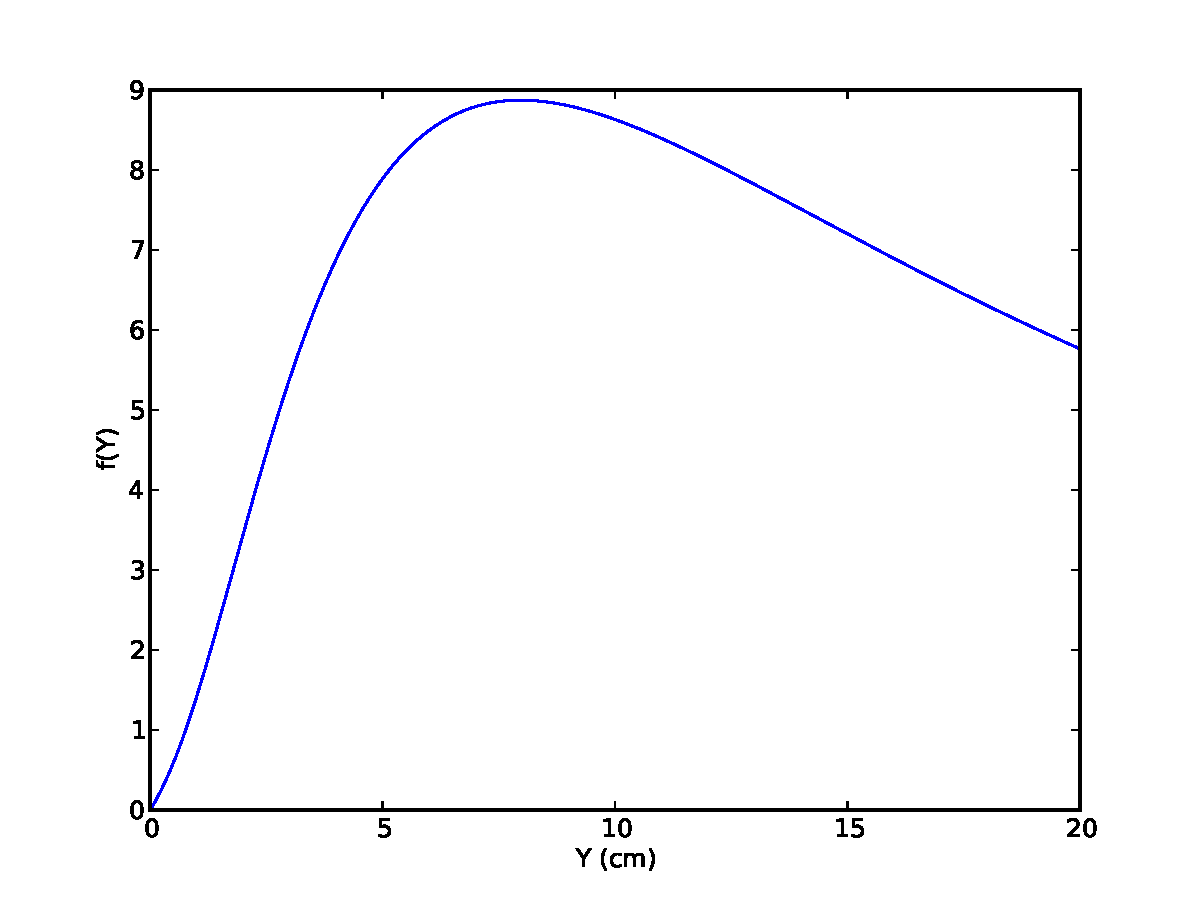
\includegraphics[width=4in]{preliminary_plot.pdf}
\end{center}

\section{Experimental Methods}
\subsection{Apparatus}
%B
\subsection{Procedures}
%E

\section{Results and Discussion}
%Ekta

\section{Conclusion}
%Brandon


\begin{thebibliography}{99}
\end{thebibliography}
\end{document}